\documentclass[10pt]{beamer}
\usetheme{metropolis}  
\usecolortheme{wolverine}
\usepackage{hyperref}
\usepackage{bigints}
\usepackage{amsmath}
\title{Introducci\'on a la probabilidad y estad\'istica CM274}
 \usepackage[spanish]{babel}
 \decimalpoint
\date{\today}
\author{C\'esar Lara Avila}
\institute{\url{https://github.com/C-Lara}}
\begin{document}
  \maketitle
  \section{5b. Varianza  de variables aleatorias discretas }
  
\begin{frame}{Difusi\'on}

\small {El valor esperado (media) de una variable aleatoria es una medida de \textcolor{red}{localizaci\'on o tendencia central}. Si tuviera que resumir una variable aleatoria con un solo n\'umero, la media ser\'ia una buena opci\'on. 

Sin embargo, la media deja fuera una buena cantidad de informaci\'on. Por ejemplo, las variables aleatorias $X$ e $Y$ tienen la media $0$, pero su masa de la probabilidad se separa de la media totalmente diferentemente.}

\vspace{0.3cm}


\begin{table}[]
	\centering
	\begin{tabular}{c|ccccc}
		valores  x & -2   & -1   & 0    & 1    & 2   \\
		\hline
		pmf p(x)   & 1/10 & 2/10 & 4/10 & 2/10 & 1/10
	\end{tabular}
\end{table} \begin{table}[]
	\centering
	\begin{tabular}{c|cc}
		valores  y & -3  & 3   \\
		\hline
		pmf p(y)   & 1/2 & 1/2
	\end{tabular}
\end{table}
\end{frame}
\begin{frame}{Difusi\'on}
\small {Probablemente sea un poco m\'as f\'acil ver los diferentes propagaciones  en las gr\'aficas de las funciones de masa de probabilidad. Utilizamos barras en lugar de puntos para dar una mejor percepci\'on de la masa. 
	
El gr\'afico siguiente es la funci\'on de masa de probabilidad para dos distribuciones con media $0$.

	
\begin{figure}[ht]
	\centering
	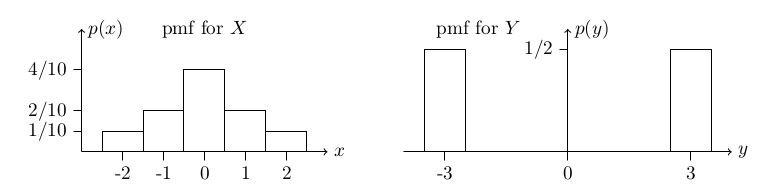
\includegraphics[scale=.4]{J1.png}
\end{figure}
	}
\end{frame}

\begin{frame}{Varianza y desviaci\'on est\'andar}
\small{Tomando la media como el centro de la distribuci\'on de probabilidad de una variable aleatoria, la varianza es una medida de cuanto la masa de probabilidad se extiende alrededor de este centro. Empezaremos con la definici\'on formal de la varianza y luego revisaremos su significado.
	
Si $X$ es una variable aleatoria con media $\mathbb{E}(X) = \mu$, entonces la \textcolor{orange}{varianza} de $X$ se define por:

\[
\text{Var}(X) = \mathbb{E}((X - \mu)^2).
\]


La \textcolor{violet}{desviaci\'on est\'andar}  $\sigma$ de $X$ es definida por

\[
\sigma = \sqrt{\text{Var}(X)}.
\]
}
\end{frame}

\begin{frame}{Varianza y desviaci\'on est\'andar}
\small{Si la variable aleatoria relevante es clara desde el contexto, entonces la varianza y la desviación est\'andar se denotan a menudo por $\sigma^2$ y $\sigma$ , as\'i como la media es $\mu$.
	
?`Qu\'e significa esto? Primero, vamos a reescribir la definici\'on expl\'icitamente como una suma. Si $X$ toma valores $x_1, x_2,\dots, x _n$  con funci\'on de masa de probabilidad $p(x_i)$ entonces
		
\[
\text{Var}(X) = \mathbb{E}((X - \mu)^2) = \sum_{i =1}^{n}p(x_i)(x_i - \mu)^2.
\]

En palabras, la f\'ormula de $\text{Var}(X)$ dice que se toma  un promedio ponderado de la distancia cuadrada a la media. Mediante la cuadratura, nos aseguramos de que estamos promediando s\'olo valores positivos, de modo que la propagaci\'on  a la derecha de la media no cancele la de la izquierda. }
\end{frame}

\begin{frame}{Varianza y desviaci\'on est\'andar}
\small{ Usando esperanza, estamos ponderando valores de probabilidad altos m\'as que valores de probabilidad bajos.

\vspace{0.3cm}
	
\textcolor{blue}{Notas sobre unidades:}


\begin{enumerate}
\item $\sigma $ tiene las mismas unidades que $X$.
\item $\text{Var}(X)$ tiene las mismas unidades que el cuadrado de $X$. As\'i que si $X$ est\'a en metros, entonces $\text{Var}(X)$ est\'a en metros al cuadrado. Debido a que $\sigma$ y $X$ tienen las mismas unidades, la desviaci\'on est\'andar es una medida natural de propagaci\'on.
\end{enumerate}
}
\end{frame}

\begin{frame}{Ejemplos}
\small{1.  Para cada variable $X, Y, Z$ y $W$ dibujamos la funci\'on de masa de probabilidad y calculamos la media y la varianza.

\begin{flushleft}
\textcolor{red}{Funci\'on de masa de probabilidad $X$}
 \begin{table}[]
 	\begin{tabular}{c|ccccc}
 		valores  x & 1   & 2   & 3    & 4    & 5   \\
 		\hline
 		pmf p(x)   & 1/5 & 1/5 & 1/5 & 1/5 & 1/5
 	\end{tabular}
 \end{table}
 \textcolor{blue}{Funci\'on de masa de probabilidad $Y$}
 \begin{table}[]
 	\begin{tabular}{c|ccccc}
 		valores  y & 1   & 2   & 3    & 4    & 5   \\
 		\hline
 		pmf p(y)   & 1/10 & 2/10 & 4/10 & 2/10 & 1/10
 	\end{tabular}
 \end{table}
 \textcolor{violet}{Funci\'on de masa de probabilidad $Z$}
 \begin{table}[]
 	\begin{tabular}{c|ccccc}
 		valores  z & 1   & 2   & 3    & 4    & 5   \\
 		\hline
 		pmf p(z)   & 5/10 & 0 & 0 & 0 & 5/10
 	\end{tabular}
 \end{table}
 
\end{flushleft}
}
\end{frame}

\begin{frame}{Ejemplos}
\begin{flushleft}
\textcolor{orange}{Funci\'on de masa de probabilidad $W$}
\begin{table}[]
	
	\begin{tabular}{c|ccccc}
		valores  w & 1   & 2   & 3    & 4    & 5   \\
		\hline
		pmf p(w)   & 0 & 0 & 0 & 0 & 0
	\end{tabular}
\end{table}
\end{flushleft}

\small{Cada variable aleatoria tiene la misma media $3$, pero la probabilidad se difunde de manera diferente. En los diagramas a continuaci\'on, mostramos los pmf de mayor a menor varianza: $Z$, $X$, $Y$, $W$.
	
	
	\begin{figure}[ht]
		\centering
		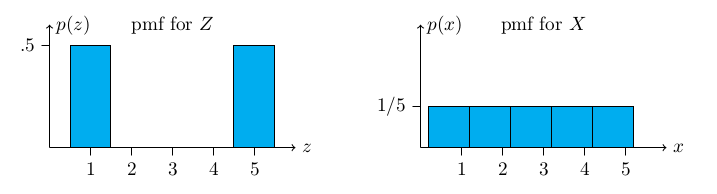
\includegraphics[scale=.35]{J2.png}
	\end{figure}	
	}
\end{frame}

\begin{frame}{Ejemplos}
\small{ 
\begin{figure}[ht]
		\centering
		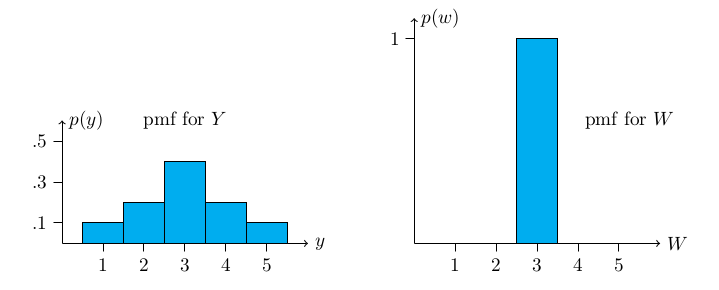
\includegraphics[scale=.35]{J3.png}
\end{figure}	

A continuaci\'on verificamos nuestra intuici\'on visual calculando la varianza de cada una de las variables. Todos ellos tienen como media $\mu = 3$. Dado que la varianza se define como un valor esperado, podemos calcularlo usando  tablas.

\vspace{0.2cm}

\begin{table}[]
 \begin{tabular}{c|ccccc}
 		valores  x & 1   & 2   & 3    & 4    & 5   \\
 		\hline
 		pmf p(x)   & 1/5 & 1/5 & 1/5 & 1/5 & 1/5 \\
 		\hline
 		(X - $\mu^2$) & 4 & 1 & 0 & 1 & 4
 	\end{tabular}
 \end{table}
	
}
\end{frame}

\begin{frame}{Ejemplos}
	\small{
\[
\text{Var}(X) = \mathbb{E}((X - \mu)^2) = \frac{4}{5} + \frac{1}{5} + \frac{0}{5} + \frac{1}{5} + \frac{4}{5} = 2
\]

\begin{table}[]
	\begin{tabular}{c|ccccc}
		valores  y & 1   & 2   & 3    & 4    & 5   \\
		\hline
		pmf p(y)   & 1/10 & 2/10 & 4/10 & 2/10 & 1/10\\
		\hline
		(Y - $\mu^2$) & 4 & 1 & 0 & 1 & 4
	\end{tabular}
\end{table}	

\[
\text{Var}(Y) = \mathbb{E}((Y - \mu)^2) = \frac{4}{10} + \frac{2}{10} + \frac{0}{10} + \frac{2}{10} + \frac{4}{10} = 1.2
\]

\begin{table}[]
	\begin{tabular}{c|ccccc}
		valores  z & 1   & 2   & 3    & 4    & 5   \\
		\hline
		pmf p(z)   & 5/10 & 0 & 0 & 0 & 5/10 \\
		\hline
		(Z -$\mu^2$) & 4 & 1 & 0 & 1 & 4
	\end{tabular}
\end{table}

\[
\text{Var}(Z) = \mathbb{E}((Z - \mu)^2) =  \frac{20}{10} +  \frac{20}{10} = 4.
\]
}
\end{frame}

\begin{frame}{Ejemplos}
\small{
\begin{table}[]
	
	\begin{tabular}{c|ccccc}
		valores  w & 1   & 2   & 3    & 4    & 5   \\
		\hline
		pmf p(w)   & 0 & 0 & 0 & 0 & 0\\
		\hline
		(W -$\mu^2$) & 4 & 1 & 0 & 1 & 4 
	\end{tabular}
\end{table}

\[
\text{Var(W) = 0}.
\]

Ten en cuenta que W no var\'ia, por lo que tiene varianza 0!.

\vspace{0.2cm}

2. Si $X \sim \text{Bernoulli}(p)$ entonces $\text{Var}(X)	= p(1 - p)$. 


En efecto, sabemos que $\mathbb{E}(X) = p$. Ahora calculamos $\text{Var}(X)$ usando una tabla.

\begin{table}[]
	
	\begin{tabular}{c|cc}
		valores  X & 0    & 1     \\
		\hline
		pmf p(x)   & 1 -p & p \\
		\hline
		(X -$\mu^2$) & $(0 - p)^2$ & $(1 -p)^2$	 
	\end{tabular}
\end{table}

}
\end{frame}

\begin{frame}{Ejemplos}
	\small{
\[
\text{Var}(X) = (1 - p)p^2 + p(1 - p)^2 = (1 - p)p(1 - p + p) = (1 - p)p
\]

Como con todas las cosas de Bernoulli, debe recordar esta f\'ormula.


\vspace{0.3cm}

\textcolor{red}{\textbf{Pregunta:}} ?` Para qu\'e valor de $p$ tiene  $\text{Bernoulli}(p)$ tiene la varianza m\'as alta?.


\vspace{4.2cm}

}

\end{frame}

\begin{frame}{Independencia}
	
\small{Hasta ahora hemos estado utilizando la noci\'on de variable aleatoria independiente sin nunca cuidadosamente definirla. Por ejemplo, una distribuci\'on binomial es la suma de ensayos independientes de Bernoulli. 
	
En un  sentido probabil\'istico  las variables aleatorias $X$ e $Y$ son independientes si conociendo el valor de $X$ no da ninguna informaci\'on sobre el valor de $Y$.
	
Por ahora podemos usar la siguiente definici\'on, que  es v\'alida para variables aleatorias discretas.
	
\textcolor{violet}{\textbf{Definici\'on:}}
	
Las variables aleatorias  discretas $X$ e $Y$ son \textcolor{orange}{independiente} si

\[
\mathbb{P}(X =a, Y = b) = \mathbb{P}(X =a)\mathbb{P}(Y = b)
\]


para valores $a, b$. Es decir, las probabilidades se multiplican.	
}
\end{frame}

\begin{frame}{Propiedades de la varianza}
	
\small{ Las tres propiedades m\'as \'utiles para calcular la varianza son:

\begin{enumerate}
	\item Si $X$ y $Y$ son \textcolor{red}{independientes} entonces $\text{Var}(X +Y) = \text{Var}(X) + \text{Var}(Y)$.
	\item Para constantes $a$ y $b$, $\text{Var}(aX + b) = a^2\text{Var(X)}.$
	\item $\text{Var}(X) = \mathbb{E}(X^2) - \mathbb{E}(X)^2$.
\end{enumerate}

Para la propiedad 1, anote cuidadosamente el requisito de que $X$ e $Y$ son independientes. 

La propiedad 3 da una f\'ormula para $\text{Var}(X)$ que a menudo es m\'as f\'acil de usar en c\'alculos manuales.
}

\end{frame}


\begin{frame}{Ejemplos}
\small{1. Usa la propiedad 3 para calcular la varianza de $X \sim \text{Bernoulli}(p).$
	
Desde la tabla,

\begin{table}[]
	
	\begin{tabular}{c|cc}
		valores  X & 0    & 1     \\
		\hline
		pmf p(x)   & 1 -p & p \\
		\hline
		$X^2$ & 0 &  1	 
	\end{tabular}
\end{table}

tenemos que $\mathbb{E}(X^2) = p$. As\'i con la propiedad 3 produce,

\[
\text{Var(X)} = \mathbb{E}(X^2) - \mathbb{E}(X)^2 = p - p^2 = p(1 -p).
\]

2. Supongamos $X \sim \text{Binomial}(n,p)$. Desde que $X$  es la suma de variable $\text{Bernoulli}(p)$ independientes y desde que cada variable de Bernoulli tiene varianza $p(1 -p)$, tenemos

\[
X \sim \text{Binomial(n,p)} \rightarrow \text{Var}(X) = np(1 - p).
\]
}
\end{frame}

\begin{frame}{Prueba de las propiedades de la varianza}
\small{ \textcolor{red}{\textbf{Prueba de la propiedad 2}}: Esto se sigue de las propiedades de $\mathbb{E}(X)$ y algo de \'algebra. Sea $\mu = \mathbb{E}(X)$. Entonces $\mathbb{E}(aX + b) = a\mu + b$ y

\begin{align*}
\text{Var}(aX + b) &= \mathbb{E}((aX + b - (a\mu + b))^2) = \mathbb{E}((aX -a\mu)^2) \\
& = \mathbb{E}(a^2(X - \mu)^2) = a^2\mathbb{E}((X - \mu)^2) = a^2\text{Var}(X).
\end{align*}


\textcolor{red}{\textbf{Prueba de la propiedad 3}}: Usamos la propiedad de $\mathbb{E}(X)$ y un poco de \'algebra. Se debe recordar que $\mu$ es una constante y que $\mathbb{E}(X) = \mu$.

\begin{align*}
\mathbb{E}((X - \mu)^2) &= \mathbb{E}(X^2 -2\mu X + \mu^2)\\
						&= \mathbb{E}(X^2) - 2\mu\mathbb{E}(X) + \mu^2 \\
						&= \mathbb{E}(X^2) - 2\mu^2 + \mu^2 \\
						&= \mathbb{E}(X^2) -\mu^2 \\
						&= \mathbb{E}(X^2) - \mathbb{E}(X)^2.
\end{align*}
}
\end{frame}
\end{document}